\documentclass[12pt,a4paper]{article}
\usepackage[utf8]{inputenc}
\usepackage[french]{babel}
\usepackage[T1]{fontenc}
\usepackage{amsmath}
\usepackage{amsfonts}
\usepackage{amssymb}
\usepackage{graphicx}
\usepackage[left=2cm,right=2cm,top=2cm,bottom=2cm]{geometry}
\usepackage[thinspace,thinqspace,amssymb]{SIunits}
\usepackage{eurosym}

\title{Mise en perspective didactique d'un dossier de recherche}
\author{Rémi Metzdorff}
\date{\today}

\renewcommand{\d}{\mathrm{d}}
\newcommand{\uroc}{\micro RoC}

%%%%%%%%%%%%%%%%%%%%%%%%%%%%%%  For CV  %%%%%%%%%%%%%%%%%%%%%%%%%%%%%%
\usepackage{array}
\newcolumntype{L}[1]{>{\raggedright\let\newline\\\arraybackslash\hspace{0pt}}m{#1}}
\newcolumntype{C}[1]{>{\centering\let\newline\\\arraybackslash\hspace{0pt}}m{#1}}
\newcolumntype{R}[1]{>{\raggedleft\let\newline\\\arraybackslash\hspace{0pt}}m{#1}}
%%%%%%%%%%%%%%%%%%%%%%%%%%%%%%%%%%%%%%%%%%%%%%%%%%%%%%%%%%%%%%%%%%%%%%

\usepackage{xcolor}
\definecolor{theme}{RGB}{56,115,179}

\begin{document}

\maketitle

%\tableofcontents

\section{Parcours universitaire et scientifique}

\noindent
\begin{tabular*}{\textwidth}{p{0.12\textwidth}<{\raggedleft}p{0.83\textwidth}}
\textcolor{theme}{\rule{0.12\textwidth}{2.5mm}} &
\large\textcolor{theme}{Formation et doctorat} \vspace{3pt} \\
2015--2019 &
\textbf{Doctorat :} Thèse en optomécanique réalisée au sein de l'équipe Optomécanique et Mesures Quantiques du laboratoire Kastler Brossel (LKB, Paris) sous la direction de Pierre-François Cohadon intitulée \textbf{Refroidissement de résonateurs macroscopiques proche de leur état quantique fondamental}, soutenue le 23 Juillet 2019. \vspace{3pt} \\
2014--2015 &
\textbf{Master 2 :} Parcours LuMI (Lumière, Matière, Interactions) du master OMP (Optique, Matière, Plasma) de l'UPMC (Paris).
Stage de recherche au LKB (6 mois) sur l'étude de l'évolution des pertes dans des cavités Fabry Perot de grande finesses en fonction de leur longueur. \vspace{3pt} \\
2013--2014 &
\textbf{Master 1 :} Parcours Physique Générale du master Physique et Applications de l'UPMC (Paris).
Stage au LKB (4 mois) sur le développement de collimateurs compacts pour les faisceaux d'un piège magnéto-optique à trois dimensions (3D-MOT) sur une expérience de métrologie. \vspace{3pt} \\
2012--2013 &
\textbf{Licence 3 :} Parcours Physique-Chimie de l'UPMC (Paris). \vspace{3pt} \\
2010--2012 &
\textbf{CPGE :} PCSI et PC$^*$ au Lycée Louis-le-Grand (Paris). \vspace{10pt} \\

\textcolor{theme}{\rule{0.12\textwidth}{2.5mm}} &
\large\textcolor{theme}{Enseignements, diffusion et vulgarisation} \vspace{3pt} \\
2015--2018 & \textbf{Monitorats :}
\begin{itemize}
\item travaux pratiques d'électromagnétisme (L1) ;
\item travaux dirigés et travaux pratiques de physique expérimentale (L2-L3) : programmation, électronique, Arduino ;
\item travaux pratiques d'optique (M1) : laser, diode laser.
\end{itemize}\\
2015--2019 &
\textbf{Conférences :} COLOQ, CLEO, ... \vspace{3pt} \\
& \textbf{Vulgarisation :}
\begin{itemize}
\item \textbf{Un chercheur, Une manip (2019) :} Présentations au Palais de la Découverte autour de la découverte des ondes gravitationnelles ;
\item \textbf{Fêtes de la science :} Présentation du LKB au grand public, conférence sur la détection d'ondes gravitationnelles, animations grand public ;
\item \textbf{E=M6 :} Casser un verre avec la voix ;
\item \textbf{Olympiades de physique :} Conférence sur la découverte des ondes gravitationnelles.
\end{itemize}
\end{tabular*}

\section{Vers l'état quantique fondamental d'oscillateurs mécaniques macroscopiques}

\subsection{Contexte : mesures de déplacements et optomécanique}

Les propriétés de la lumière en font un outil de choix pour de nombreuses mesures de déplacements, à commencer par la définition actuelle du mètre qui se base directement sur la célérité de la lumière.
La mesure de la \textbf{distance absolue} Terre-Lune repose par exemple sur la détermination du temps de vol d'impulsions lumineuses permettant des incertitudes relative de l'ordre de $10^{-9}$.
Le développement de techniques interferométriques autorise par ailleurs les \textbf{mesures relatives} les plus sensibles réalisées actuellement (ces techniques ne se cantonnent pas à l'utilisation de lumière mais exploitent également le comportement ondulatoire d'ensembles d'atomes pour fabriquer par exemple les horloges les plus stables jamais créées, avec des incertitudes relatives de l'ordre de $10^{-15}$ pour les horloges au césium et jusqu'à $10^{-18}$ pour celles à l'ytterbium).
Une des applications majeures de l'interférométrie optique est la détection des ondes gravitationnelles au moyen d'interféromètres géants comme celui du projet Virgo (situé à Cascina, près de Pise) ou LIGO (Hanford et Livingston, États-Unis).
Les développements considérables des dernières décennies ont permis pour la première fois, 100 ans après leur prédiction par A. Einstein, l'observation directe d'ondes gravitationnelles issues de la coalescence de deux trous noirs de quelques dizaines de masses solaires et situés à plus de $10^6$ années lumières.
L'amplitude maximale du signal mesuré sur Terre était alors proche de $\unit{10^{-21}}{\meter\per\sqrt{\hertz}}$ (soit un déplacement de $\unit{10^{-18}}{\meter}$) ce qui en faisait le signal le plus faible jamais détecté associé à l'évènement le plus violent jamais observé.

Ces détecteurs sont des interféromètres de Michelson géants dont les bras sont replacés par des cavités Fabry Perot pour augmenter l'effet d'un petit déphasage (la longueur des bras de Virgo est de \unit{3}{\kilo\meter}, avec des cavités de finesse 50).
Le passage d'une onde gravitationnelle introduit un déphasage qui peut être mesuré à la sortie de l'appareil comme des variations de l'intensité lumineuse transmise par le Michelson.
Toute perturbation du détecteur se traduit donc comme un bruit qui, inévitablement, dégrade la sensibilité de la mesure : par exemple, le bruit sismique agite directement les miroirs qui doivent donc être isolés grâce à un système complexe d'atténuateurs permettant une réduction du bruit d'un facteur $10^{14}$, pour se rapprocher du cas idéal de masses libres.
Le bruit thermique au niveau des miroirs se traduit directement sous la forme d'un mouvement Brownien qui conduit à utiliser des matériaux (silice) et des géométries permettant de concentrer les fluctuations de position autour des fréquences propres du système.
La réduction de ces sources de bruit classique est maintenant telle que des bruits quantiques liés au laser lui même deviennent limitant.
Le \textbf{bruit quantique de phase} se traduit directement sur la mesure puisque ses fluctuations sont décorrélées entre les deux bras de l'interféromètre.
Il peut être réduit en augmentant l'intensité du laser ce qui explique l'utilisation de puissances optiques importantes ($\sim \unit{100}{\kilo\watt}$ dans les cavités).
D'autre part, le \textbf{bruit quantique d'intensité} a deux conséquences sur la sensibilité de la mesure : un bruit direct sur l'intensité mesurée à la sortie du détecteur et des fluctuations de la force de \textbf{pression de radiation} qui s'exerce sur les miroirs de l'interféromètre et qui se traduit en bruit de position, dont l'intensité augmente avec la puissance lumineuse incidente.
C'est l'action en retour de la mesure, prédite depuis les années 80, qui a contribué à lancer les recherches autour de l'optomécanique.
Le bruit de pression de radiation étant modulé par la réponse mécanique du système, il en résulte un compromis à l'origine de la limite quantique standard : à chaque fréquence correspond une puissance laser optimale qui égalise le bruit de pression de radiation et le bruit de phase.

Si l'effet de la pression de radiation peut s'avérer néfaste pour la sensibilité des mesures de grande précision, on peut également l'exploiter pour contrôler les degrés de liberté mécanique d'un miroir mobile.
C'est ainsi qu'au cours des vingt dernières années, de nombreux systèmes optomécaniques ont été développés avec des applications très variées (capteurs de force, de masse, de température, transducteurs optique-microonde, ponderomotive squeezing, etc.).
Une des applications fondamentales de ces systèmes est l'observation d'effets quantiques sur des objets de plus en plus massifs, avec notamment l'observation du premier refroidissement vers l'état quantique fondamental d'un oscillateur mécanique (de masse effective $m_\mathrm{eff} = \unit{50}{pg}$) couplé à une cavité microonde en 2011.
A travers l'utilisation d'oscillateurs mécaniques de masses effectives intermédiaires ($m_\mathrm{eff} \approx \unit{100}{\micro\gram}$), l'objectif de ma thèse était donc double :
\begin{enumerate}
\item \textbf{Refroidir un oscillateur mécanique macroscopique dans son état quantique fondamental}, avec trois ordres de grandeur de plus que les précédentes expériences, et en particulier proche de la masse de Planck ($m_\mathrm{P}=\unit{22}{\micro\gram}$) où des effets de décohérence liés à la gravité sont attendus ;
\item Préparer un système modèle qui permette d'\textbf{étudier les limites de sensibilité de la mesure de petits déplacements liés au bruit de pression de radiation}, tout en restant beaucoup plus compact que les interféromètres gravitationnels et leur miroirs ($m_\mathrm{eff}\approx\unit{50}{\kilo\gram}$).
\end{enumerate}
Le premier point est un pré-requis du deuxième puisque le système étudié est limité par le bruit thermique : afin d'observer le bruit de pression de radiation, il est nécessaire de réduire le mouvement Brownien de près de 6 ordres de grandeurs, ce qui revient à refroidir l'oscillateur mécanique proche de son état quantique fondamental.

\subsection{L'oscillateur mécanique, caractérisation et thermométrie}

\begin{figure}
\center
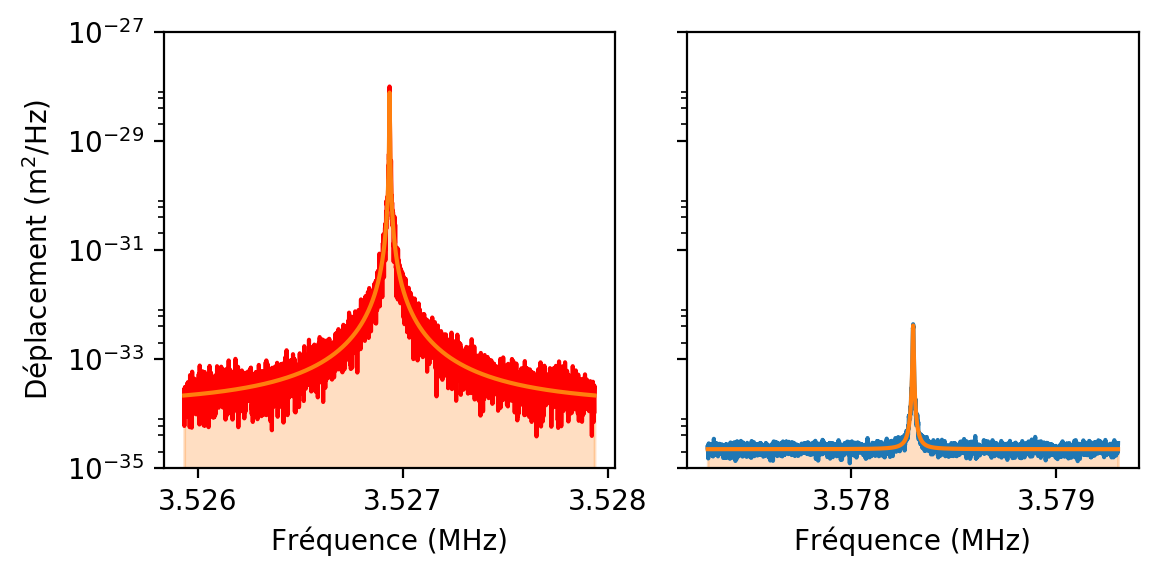
\includegraphics[scale=0.75]{figures/thermal_peak_def_filled.png}
\caption{Spectres du bruit de position d'un micro-pilier en cavité dû au mouvement Brownien de l'oscillateur.
La figure de gauche est obtenue à température ambiante alors que celle de droite est obtenue en cryogénie à \unit{30}{\milli\kelvin}.
Le refroidissement de l'échantillon s'accompagne d'un déplacement de sa fréquence de résonance, d'une augmentation de son facteur de qualité et d'une diminution de l'aire sous le pic, proportionnelle à la température.}
\end{figure}

Bien que les géométries des oscillateurs mécaniques soient très variées, son comportement est très bien décrit par un système \{masse, ressort\} amorti ($m_\mathrm{eff}$, $\Omega_m$, $\Gamma_m$) soumis à des forces extérieures de résultante $F_\mathrm{ext}$
\begin{equation}
m_\mathrm{eff} \frac{d^2 x(t)}{\d t^2} + m_\mathrm{eff}\Gamma_m \frac{d x(t)}{\d t} + m_\mathrm{eff} \Omega_m^2 x(t) = F_\mathrm{ext}(t).
\end{equation}
Son comportement fréquentiel se déduit dans l'espace de Fourier de la susceptibilité mécanique $\chi[\Omega]$ de l'oscillateur 
\begin{equation}
\chi[\Omega] = \frac{1}{m_\mathrm{eff}[(\Omega_m^2-\Omega^2)-i\Gamma_m\Omega]},
\end{equation}
où $i^2=-1$. 
Dans la théorie de Langevin, le terme de dissipation $\Gamma_m$ se traduit par un couplage de l'oscillateur à son environnement assimilé à un bain thermique à la température $T_\mathrm{env}$.
Il en résulte une force $F_T$, dont le spectre est lié à la partie imaginaire de la susceptibilité mécanique par le théorème de fluctuations-dissipations, à l'origine du mouvement Brownien de l'oscillateur.
On peut ainsi montrer que le spectre de déplacement du résonateur à l'équilibre thermodynamique avec un tel bain thermique est directement lié au rapport $T_\mathrm{env}/m_\mathrm{eff}$ : la connaissance de l'un permet donc de déterminer l'autre à travers la mesure du spectre du mouvement Brownien du résonateur.
Le spectre est aussi d'autant plus piqué autour de la fréquence propre $\Omega_m$ que la dissipation est faible, ce qui conduit à utiliser des oscillateur avec des facteurs de qualité mécaniques $Q=\Omega/\Gamma_m$ très élevés.
\emph{En accord avec le programme de première année de CPGE, cette approche classique peut illustrer un exercice de mécanique, avec l'étude de l'oscillateur harmonique amorti, en régime libre ou forcé.
La mesure des différents paramètres de l'oscillateur permet également d'en faire un capteur de grande précision.
L'évolution de l'amortissement peut être reliée à la viscosité d'un fluide dans lequel est plongé l'oscillateur, celle de la fréquence relié à la masse effective pour obtenir une balance, etc. ce qui offre autant d'exemples qui pourraient illustrer un problème.
La description fréquentielle de la réponse mécanique pourrait aussi être rapprochée de l'étude de filtres électroniques pour comprendre par exemple le fonctionnement des systèmes ressort/pendules des suspensions de Virgo.}

Cette description classique ne permet cependant pas d'expliquer le comportement de l'oscillateur aux très basses températures.
Il est alors nécessaire d'utiliser un modèle quantique, où l'Hamiltonien du système est simplement celui d'une masse $m_\mathrm{eff}$ dans un puits de potentiel à une dimension de pulsation $\Omega_m$.
La résolution de l'équation de Schrödinger conduit à une quantification des niveaux d'énergie du système sous forme de demi-entiers de $\hbar\Omega_m$.
L'état du système peut alors être décrit en terme de niveau d'occupation exprimé en nombre de phonons $n_\mathrm{T}$
\begin{equation}
n_\mathrm{T} = \left[ e^\frac{T_Q}{T} -1\right]^{-1} \underset{T\gg T_Q}{\approx} \frac{T}{T_Q},
\end{equation}
où la température quantique $T_Q$ est définie comme $T_Q = \hbar\Omega_m/k_B$.
En particulier, l'énergie minimale du système dans son état fondamental n'est pas nulle et conduit à un bruit de position appelé fluctuations de point zéro d'amplitude $x_\mathrm{ZPF}$ donnée par
\begin{equation}
x_\mathrm{ZPF}=\sqrt{\frac{\hbar}{2m_\mathrm{eff}\Omega_m}}.
\end{equation}
L'objectif de ma thèse peut alors être précisé puisqu'il s'agit de refroidir un résonateur mécanique à une température inférieur à $T_Q$ pour laquelle le niveau d'occupation est inférieur à un phonon.
\emph{Cette description quantique rentre complètement dans le cadre du programme de la deuxième année de CPGE.}

\begin{figure}
\center
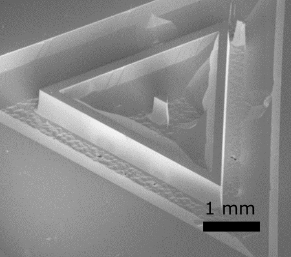
\includegraphics[height=90pt]{figures/micropillar.png}
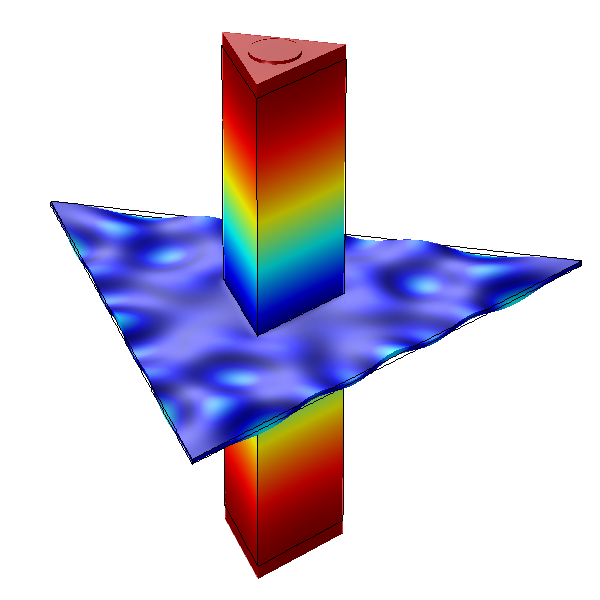
\includegraphics[height=90pt]{figures/micropillar_disp.png}
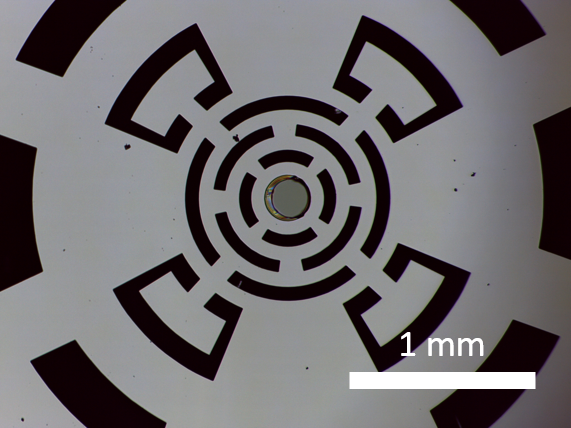
\includegraphics[height=90pt]{figures/microwheel.png}
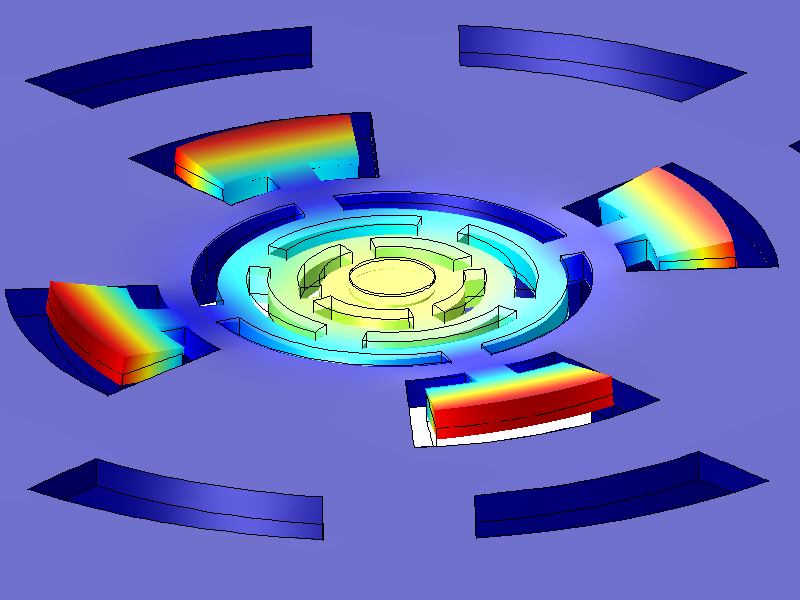
\includegraphics[height=90pt]{figures/microwheel_disp.png}
\caption{A gauche : image obtenue par microscopie électronique d'un micro-pillier en quartz et simulation du mode propre fondamental de compression utilisé.
A droite : image obtenue par microscopie optique d'un micro-disque en silicium et simulation du mode propre utilisé.
Les simulations sont réalisées avec COMSOL (simulation par élément fini) et le code couleur correspond au déplacement de la structure.}
\label{fig:resonators}
\end{figure}

Au cours de ma thèse, j'ai utilisé deux types d'échantillons visibles sur la figure~\ref{fig:resonators} :
\begin{itemize}
\item \textbf{micro-pilier} : un oscillateur en quartz (micro-fabriqué en collaboration avec l'ONERA, Paris) sous la forme d'un pilier de section triangulaire (\unit{240}{\micro\meter} de côté, \unit{1}{\milli\meter} de long), suspendu en son centre par une membrane d'environ \unit{10}{\micro\meter} d'épaisseur, au sommet duquel est déposé un micro-miroir de très haute réflectivité (en collaboration avec le LMA, Lyon), $m_\mathrm{eff}=\unit{33,5}{\micro\gram}$, $\Omega_m=2\pi\times\unit{3,6}{\mega\hertz}$ et $Q=10^7$ : $T_{Q,\mathrm{pilier}} = \unit{200}{\micro\kelvin}$ ;
\item \textbf{micro-disque} : un disque en silicium (en collaboration avec l'UniFI, Italie) d'environ $\unit{200}{\micro\meter}$ de diamètre sur lequel est déposé un miroir de très haute réflectivité, $m_\mathrm{eff}=\unit{112}{\micro\gram}$, $\Omega_m=2\pi\times\unit{280}{\kilo\hertz}$ et $Q=10^6$ : $T_{Q,\mathrm{disque}} = \unit{10}{\micro\kelvin}$.
\end{itemize}
Avant d'être utilisés pour les expériences de refroidissement, les échantillons doivent être caractérisés soigneusement, notamment pour la thermométrie à basse température.
Il est donc nécessaire de calibrer proprement leur réponse fréquentielle à une excitation mécanique réalisée à l'aide d'une cale piézoélectrique par exemple (observation des différents modes mécaniques, mesure de $\Omega_m$, $Q$) et leur masse effective $m_\mathrm{eff}$ en mesurant le mouvement Brownien de l'oscillateur à température ambiante où la température est facilement mesurable.
On peut pour cela utiliser l'échantillon comme l'un des miroirs d'un interféromètre de Michelson, où d'une cavité Fabry Perot pour mesurer ses déplacements.
Les paramètres $\Omega_m$ et $Q$ dépendent fortement du régime de température et de pression  : l'échantillon est donc placé dans un cryostat à circulation d'hélium permettant d'atteindre rapidement des températures de l'ordre du kelvin et des pressions inférieures à $\unit{10^{-5}}{\milli bar}$.
\emph{Tout en fournissant une illustration pratique à l'approche théorique précédente, les principes des techniques employées pour la caractérisation de nos échantillons peuvent sans difficulté être utilisés pour, par exemple, la caractérisation mécanique d'un diapason en TP.
On peut ainsi s'intéresser à la méthode du ringdown (évolution libre de l'oscillateur après arrêt soudain d'une excitation) pour la mesure du facteur de qualité, où encore à des mesure de fonction de transfert mécanique, en s'appuyant éventuellement sur l'utilisation de RedPitaya comme analyseur de réseau à bas coût comme on le verra plus tard.
L'évolution des grandeurs caractéristiques du système peut alors être discutée en fonction de paramètres comme la température, la masse, effective, l'amortissement, etc.}

\subsection{Cavité optique : sensibilité et couplage optomécanique}

Comme on l'a vu, la mesure des déplacements de l'oscillateur est réalisée par interférométrie optique.
L'utilisation d'une cavité de grande finesse $\cal{F}$ permet d'amplifier de déphasage $\delta\varphi$ associé à un déplacement $\delta x$ d'un facteur $2\cal{F}$ par rapport à un simple interféromètre de Michelson :
\begin{equation}
\delta \varphi = 8\pi{\cal{F}}\frac{\delta x}{\lambda}.
\end{equation}
Ces modulations de phase se font principalement à la pulsation propre $\Omega_m$ de l'oscillateur mécanique et sont ainsi responsable de la création de bandes latérales de part et d'autre de la pulsation $\omega_\mathrm{L}$ du laser, aux fréquences $\omega_\mathrm{L} \pm \Omega_m$.
Plusieurs méthodes permettent ensuite de traduire ce déphasage en un signal mesurable à l'aide d'un analyseur de spectre par exemple :
\begin{itemize}
\item \textbf{détection directe} : si la cavité est désaccordée par rapport au laser, une variation de sa longueur est directement responsable de variations de l'intensité intracavité.
Le déplacement de l'oscillateur est ainsi relié à l'intensité réfléchie par la cavité ;
\item \textbf{détection homodyne} : si la cavité est résonante avec le laser, aucune variation d'intensité n'est mesurable directement mais la variation $\delta \varphi$ est alors maximale.
En faisant interférer le faisceau réfléchi par la cavité avec un faisceau de référence dans un interféromètre de Michelson, on observe alors les variations de l'intensité transmise par l'interféromètre.
L'utilisation d'une détection balancée permet d'atténuer fortement le bruit classique autorisant des mesures limitées par les bruits quantiques ;
\item \textbf{Pound-Drever-Hall (PDH)} : une modulation de phase de fréquence supérieure à la bande passante de la cavité est appliquée au faisceau laser incident à l'aide d'un modulateur électro-optique, créant ainsi des bandes latérales de part et d'autre de la fréquence du laser, la cavité étant maintenue résonante avec la porteuse.
Les bandes latérales sont réfléchies par le miroir d'entrée de la cavité et servent ainsi de référence de phase.
Après démodulation du signal réfléchi par la cavité on obtient une fois de plus un signal lié aux fluctuations de longueur de la cavité ;
\item \textbf{détection hétérodyne} : les précédents schémas de détection présentent l'inconvénient de replier le spectre sur les fréquences positives.
En utilisant un faisceau de référence à une fréquence $\omega_\mathrm{L}'$ différente de celle du faisceau interagissant avec la cavité, on obtient un battement autour duquel les bandes latérales mécaniques $\pm \Omega_m$ sont individuellement détectables. 
\end{itemize}
\textit{Les détections PDH et hétérodynes peuvent êtres rapprochées des méthodes de traitement du signal employées dans les télécommunications et faire l'objet d'une approche documentaire.
Les spectres obtenus peuvent faire l'objet d'une analyse qualitative afin d'illustrer les protocoles de modulation et démodulation de l'information.}

Compte tenu de la faible dimension des miroirs plans déposés sur les oscillateurs mécaniques, il est nécessaire d'utiliser comme miroir d'entrée de la cavité un miroir avec un rayon de courbure de l'ordre du millimètre (\uroc).
J'ai ainsi fabriqué par photoablation multiple à l'aide d'un laser $\mathrm{CO_2}$ des structures concaves, d'environ $\unit{200}{\micro\meter}$ de diamètre, avec des rayons de courbures et des ellipticités variés.
Un dépôt diélectrique de couches de silice $\mathrm{SiO_2}$ et oxyde de tantale $\mathrm{Ta_2O_5}$ réalisé au Laboratoire des Matériaux Avancés (Lyon) permet ensuite d'obtenir des miroirs ayant une transmission bien contrôlée entre 0 et $\unit{120}{ppm}$ typiquement.
J'ai ensuite développé un ensemble de pièces mécaniques en cuivre de haute pureté permettant un assemblage et un alignement rapide d'une cavité de $\unit{100}{\micro\meter}$ de longueur, constituée d'un échantillon (micro-pilier ou micro-disque) et d'un \uroc\ comme miroir d'entrée, qui permet un asservissement de la longueur de cavité sur le laser et compatible avec une utilisation dans un cryostat à dilution.
\textit{Avant de faire réaliser les pièces à notre atelier de fabrication mécanique, des prototypes imprimés en 3D ont été réalisés pour s'assurer de la cohérence du dessin.
L'impression 3D nous a aussi permis de fabriquer rapidement des pièces plus ou moins permanentes.
L'utilisation de ces ressources (DAO et impression 3D) permettent de mettre en place des activités à bas coût avec un matériel restreint.}

\textit{Dans notre expérience, d'autres cavités optiques sont utilisées : cavité du laser Nd\string:YAG source de tous les faisceaux utilisés, cavité de filtrage permettant de diminuer les bruits classiques du laser et cavité de mesure.
Toutes ces application permettraient de mettre en évidence différents aspects du comportement d'une cavité Fabry Perot.}

L'intensité intracavité dépend fortement du désaccord entre le laser et la cavité.
De cette manière une petite variation de la longueur de la cavité se traduit non seulement par une variation du phase du faisceau réfléchi mais aussi par une modification de la puissance incidente sur les miroirs.
Il en résulte une modulation de la pression de radiation exercée sur les miroirs qui peut en retour modifier la longueur de la cavité : c'est le \textbf{couplage optomécanique} qui peut être exploité pour le refroidissement d'un mode mécanique de l'oscillateur mécanique.

\subsection{Le refroidissement par pression de radiation}

\begin{figure}
\center
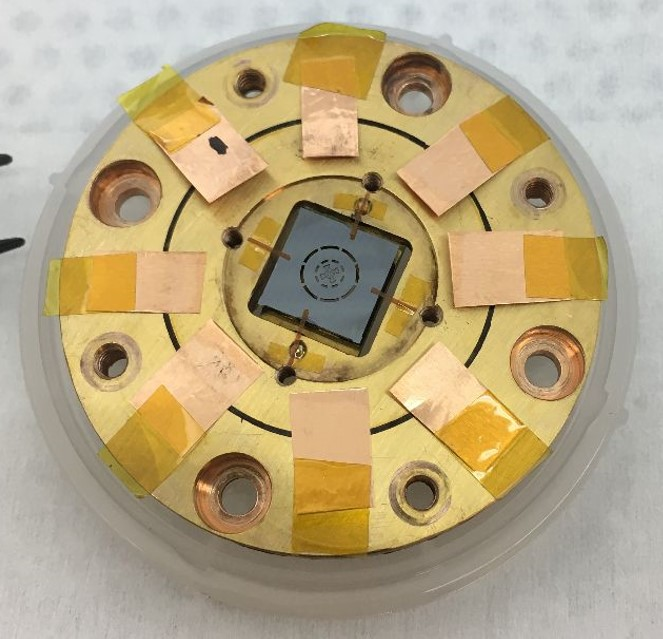
\includegraphics[height=130pt]{figures/cavity_microwheel.jpg}
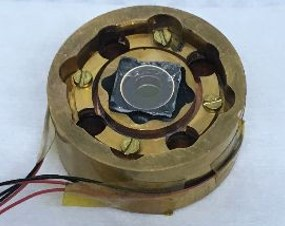
\includegraphics[height=130pt]{figures/cavity_uroc.jpg}
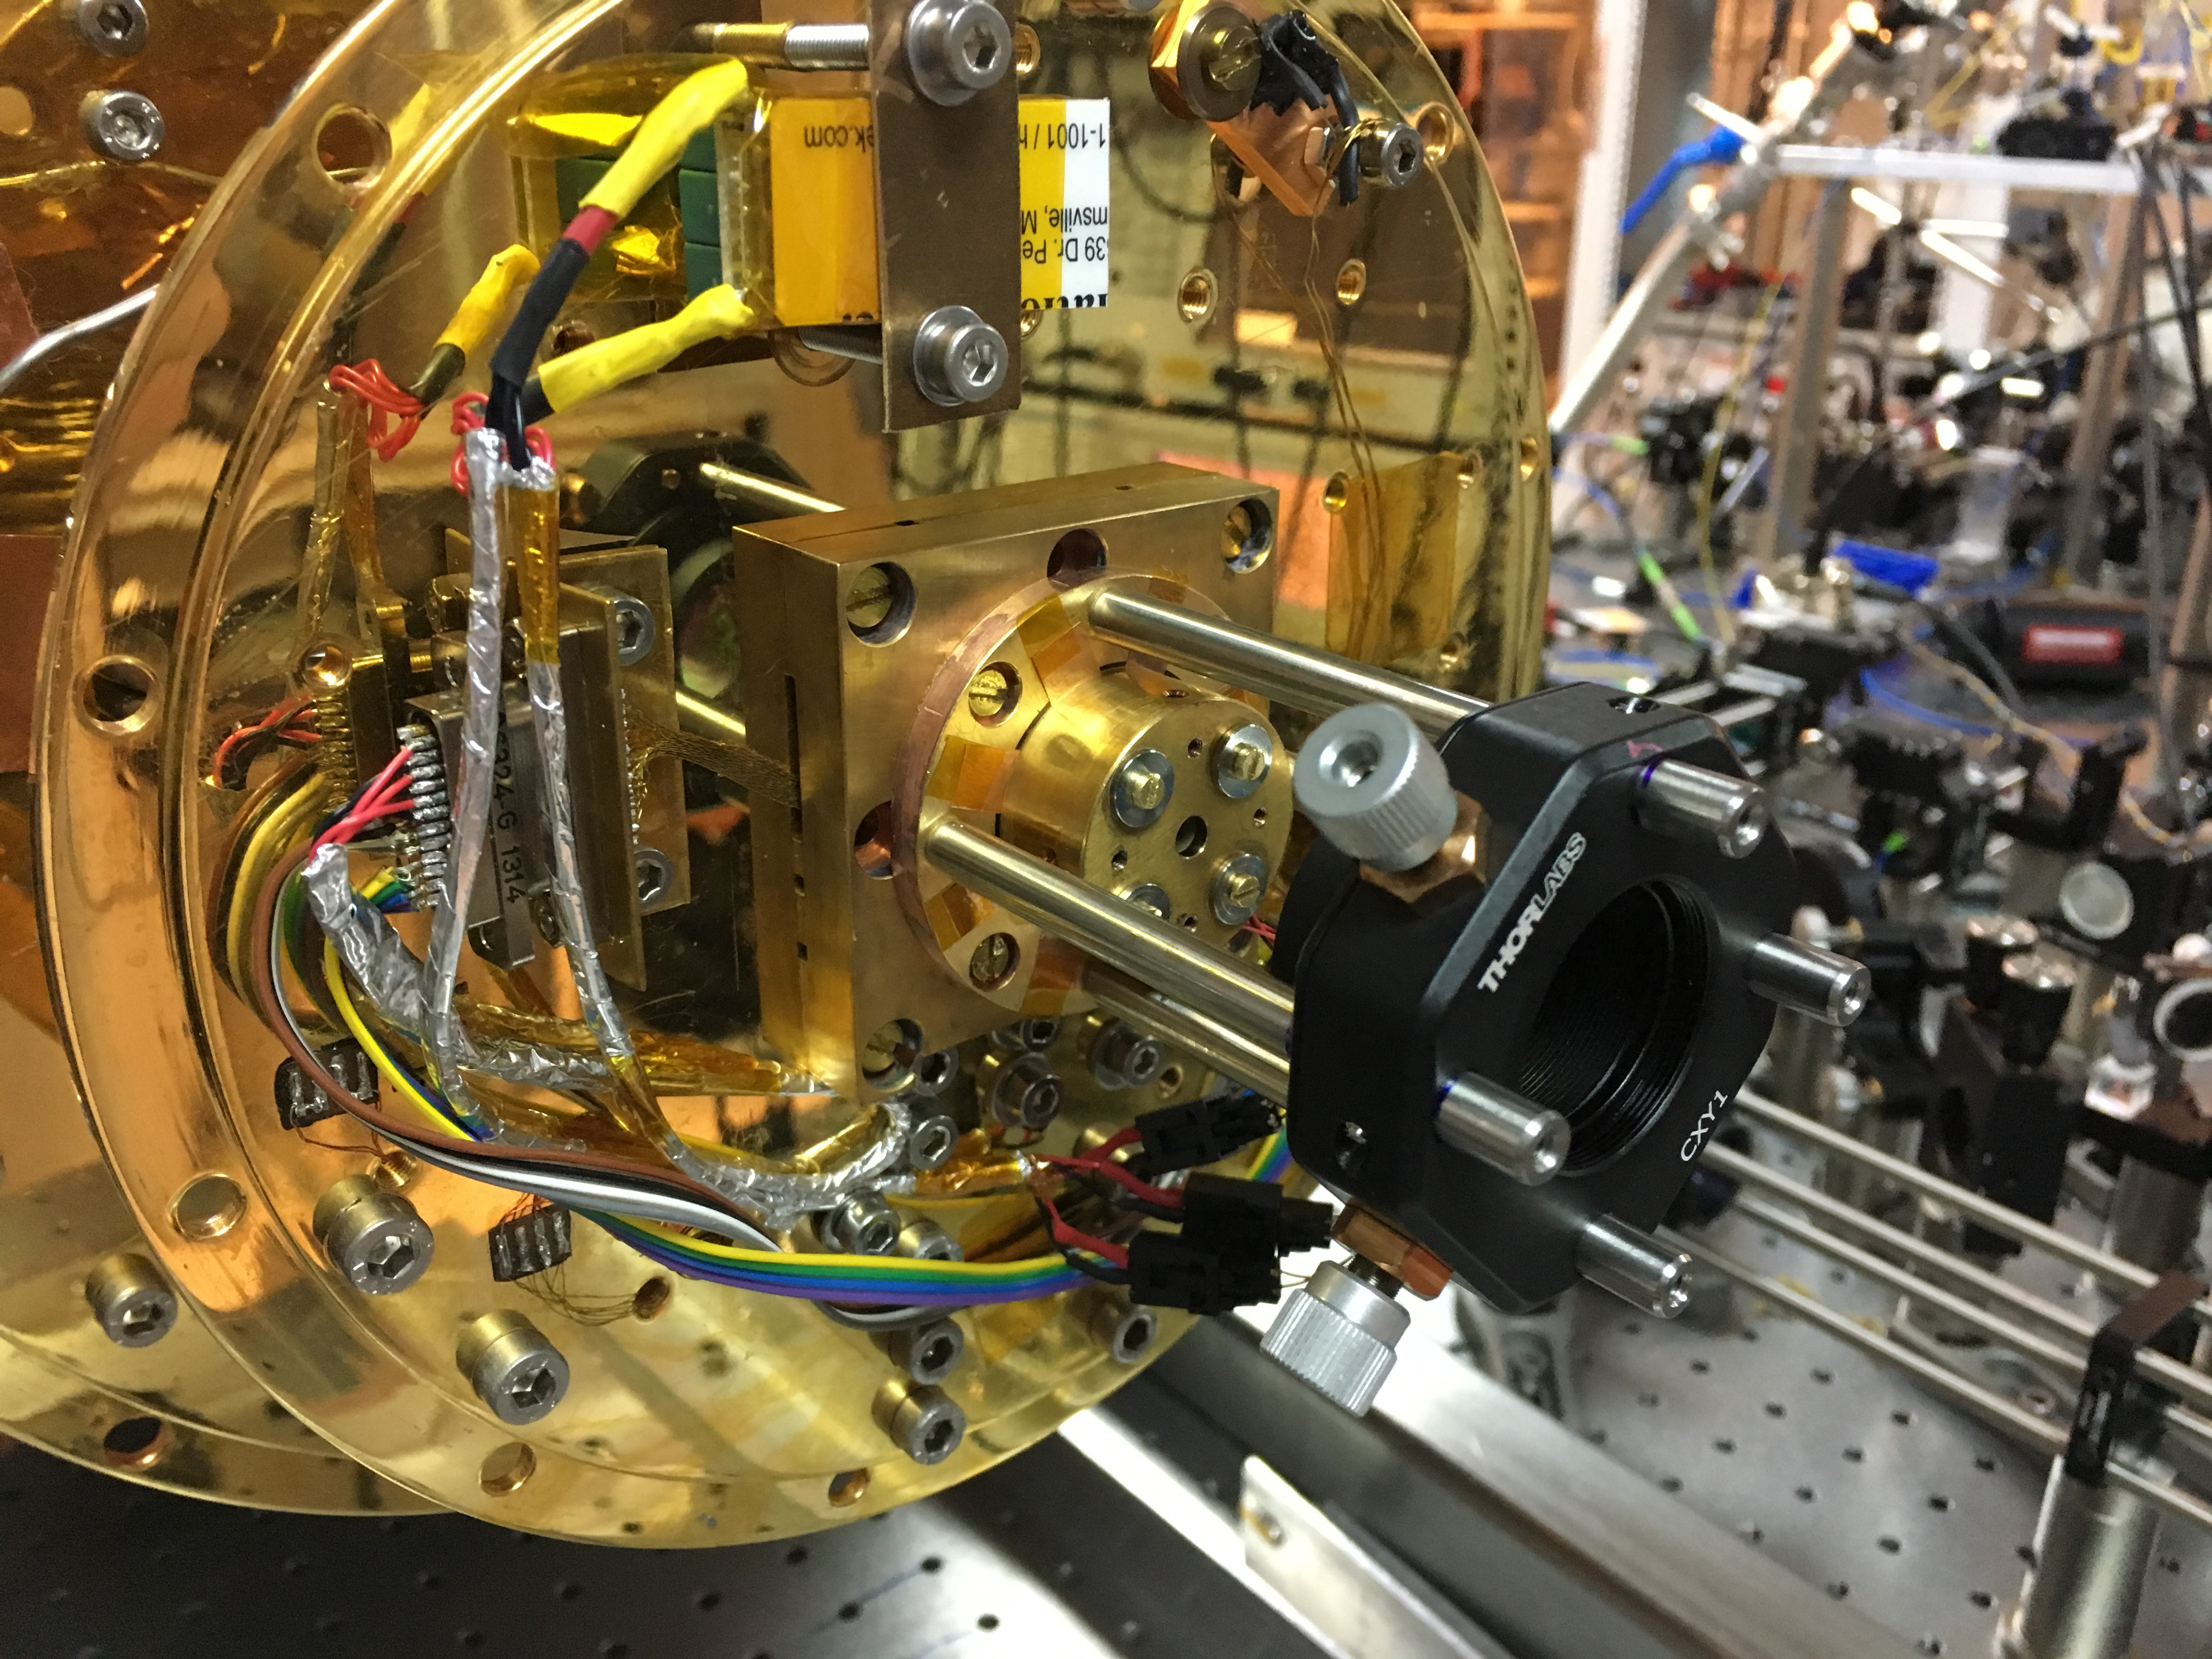
\includegraphics[height=130pt]{figures/IMG_1766.JPG}
\caption{A gauche : un échantillon micro-disque dans la première moitié de la cavité.
Au centre : le miroir de couplage (\uroc) monté dans la deuxième partie de la cavité.
Les fils permettent de contrôler les cales piézoélectriques qui permettent l'asservissement en longueur de la cavité.
A droite : photographie de la cavité de mesure assemblée et montée sur le dernier étage du cryostat à dilution.
La lentille de courte focale permet de coupler le faisceau incident au mode fondamental $\mathrm{TEM_{00}}$ de la micro-cavité.}
\end{figure}

Pour préparer les oscillateurs mécaniques dans leur état quantique fondamental, il est nécessaire d'atteindre des températures inférieures au mK.
L'utilisation d'un cryostat à circulation d'hélium permet de refroidir les échantillons à une température de quelques Kelvin suffisante pour une caractérisation préliminaire de leurs caractéristiques mécaniques, mais trop élevée pour espérer atteindre le régime quantique.
C'est donc à l'aide d'un cryostat à dilution fonctionnant avec un mélange $\mathrm{^4He/^3He}$ que la cavité de mesure est tout d'abord refroidie jusqu'à \unit{30}{\milli\kelvin}.
\textit{Le fonctionnement de ces machines thermiques peut être abordé dans le cadre d'une approche thermodynamique simplifiée.
Les problématiques liées à la conception du cryostat dans les phases préliminaires de l'expérience (enceinte sous vide, utilisation de matériaux de conductivités thermiques adaptées, accès optiques limitant le chauffage par rayonnement du corps noir) peuvent servir à illustrer les différents transferts thermiques qu'il est nécessaire de maitriser pour obtenir ces températures cryogéniques.}

Pour refroidir d'avantage l'oscillateur mécanique, il est possible d'exploiter la pression de radiation.

\subsubsection{Self-cooling}

Dans une cavité optique désaccordée, le couplage optomécanique est responsable de deux effets qui affectent le comportement mécanique de l'oscillateur : 
\begin{itemize}
\item \textbf{optical spring effect}, ou ressort optique ;
\item \textbf{cold damping}, ou friction froide.
\end{itemize}
Le premier se traduit par une modification de la constante de raideur effective de l'oscillateur qui déplace sa fréquence de résonance suivant le signe du désaccord.
Le deuxième, lié au retard de la réponse de la cavité à une modification de sa longueur, se traduit par un changement de la force de pression de radiation en quadrature de phase avec les déplacements du miroir qui donne un terme de frottement visqueux modifiant le taux d'amortissement mécanique de l'oscillateur $\Gamma_\mathrm{eff} = \Gamma_m + \Gamma_\mathrm{opt}$.
Ce terme de dissipation apparait sans ajout de bruit car le niveau d'occupation thermique du mode optique est très proche de zéro ($T_Q^\mathrm{opt}=\unit{10^4}{\kelvin}$), ce qui permet de refroidir le mode mécanique.
La température effective dépend alors du rapport entre le taux d'amortissement intrinsèque de l'échantillon $\Gamma_m$ et $\Gamma_\mathrm{eff}$ :
\begin{equation}
T_\mathrm{eff} = \frac{\Gamma_m}{\Gamma_\mathrm{eff}} T_\mathrm{env}.
\end{equation}

L'approche quantique de cet effet correspond au refroidissement par bande latérale (sideband cooling) : de part et d'autre de la fréquence du laser, les bandes latérales mécaniques dues aux échanges de phonons $\hbar\Omega_m$ entre le laser et l'oscillateur mécanique sont associées au processus Stokes (émission d'un phonon par l'oscillateur) et anti-Stokes (absorption).
En choisissant un désaccord entre le laser et la cavité égal à la fréquence mécanique, il est possible de favoriser l'un des deux processus et ainsi de refroidir (ou exciter) l'oscillateur mécanique. 

La friction froide dépend de l'intensité du faisceau incident et les précédentes expériences utilisant le micro-pilier étaient essentiellement limitées par la puissance optique injectable dans la cavité sans déclencher d'instabilité (en raison d'effets photothermiques notamment).

\subsubsection{Feedback-cooling (refroidissement par rétroaction)}

\begin{figure}
\center
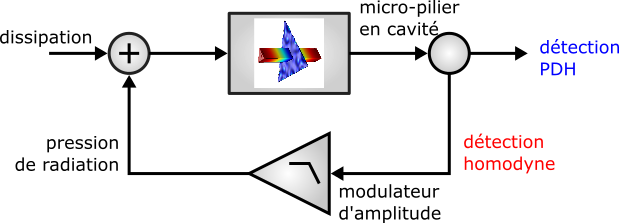
\includegraphics[scale=0.5]{figures/feedback_cooling.png}
\caption{Schéma de principe du refroidissement par rétroaction.
Le couplage à un bain thermique $T_\mathrm{env}$ en raison de la dissipation mécanique $\Gamma_m$ de l'oscillateur se traduit par un mouvement brownien du micro-pilier, qui peut être détecté optiquement en exploitant la réponse de la cavité résonante (ici grâce à une détection homodyne).
Le signal obtenu est amplifié, filtré, et alimente un actuateur (ici un modulateur d'amplitude) qui agit sur le pilier (par l'intermédiaire de la pression de radiation).
Une mesure indépendante de la boucle de rétroaction est obtenue grâce à la détection PDH.}
\end{figure}

En mesurant les fluctuations de longueur de la cavité, il est aussi possible de rétroagir sur la position de l'oscillateur.
On peut ainsi appliquer une force, proportionnelle à la vitesse de l'oscillateur, qui comme la friction froide pourra refroidir le mode mécanique de l'échantillon.
Il est alors possible de choisir les paramètres de la boucle de rétroaction pour amplifier et filtrer le bruit de position de manière à refroidir l'échantillon.

Dans l'expérience, la mesure des déplacements de l'oscillateur est réalisée grâce à une détection homodyne 


\subsection{Contrôle de l'expérience : Arduino, RedPitaya et Python}

Le fonctionnement de l'expérience repose sur plusieurs asservissements :
\begin{itemize}
\item \textbf{noise-eater} pour la réduction du bruit classique d'intensité du laser ;
\item \textbf{cavité de filtrage}, asservie en longueur sur la fréquence du laser et stabilisation de température ;
\item \textbf{oscillateur local} : asservissement à mi-frange des Michelson de la détection homodyne et hétérodyne ;
\item \textbf{intensité} des faisceaux utilisés pour les mesures ;
\item \textbf{température} des cryostats ;
\item \textbf{cavité de mesure}, asservie en longueur sur le laser ;
\item \textbf{boucle de rétroaction pour le refroidissement}.
\end{itemize}
La plupart de ces asservissements sont réalisés avec des micro contrôleurs RedPitaya et la bibliothèque PyRPL (Python RedPitaya Lockbox), développée au sein de l'équipe.
Il est ainsi possible de piloter une grande partie de l'expérience depuis un PC, ce qui autorise grâce à un répertoire de scripts Python l'automatisation des séquences de mesures.
\textit{L'utilisation, l'amélioration et le développement de ces systèmes bouclés m'a permis de développer une compréhension par l'expérience de ces systèmes asservis, renforcée par la suite par une approche plus théorique.
L'utilisation quotidienne du langage Python me donne également une certaine aisance avec cet outil.
L'utilisation de PyRPL et RedPitaya offre de nombreuses possibilités : grâce à une carte RedPitaya ($\sim\unit{200}{\text{\euro}}$) et du programme PyRPL (open source), on peut disposer d'un oscilloscope, d'un GBF, d'un analyseur de spectre, d'un analyseur de réseau et d'une lockbox (pour ne citer que les fonctionnalités déjà existantes). L'utilisation de cette ressource me semble complètement pertinente dans le cadre de travaux pratiques, à plusieurs niveaux.}

Un expérience préliminaire à la réalisation des micro-cavités de mesure nécessitait de réaliser une cavité de longueur variable sur l'ensemble de sa zone de stabilité afin d'étudier les mécanismes de pertes optique dans une cavité de grande finesse.
On a donc choisit de monter un des deux miroirs sur une translation micrométrique motorisée par un moteur pas à pas.
En vue d'automatiser les mesures, j'ai développé un contrôleur basé sur une carte Arduino (programme Arduino, interface Python et électronique) permettant le positionnement de la translation.

Filtre actifs et passifs, AOP etc

\subsection{Principaux résultats obtenus}



\begin{figure}
\center
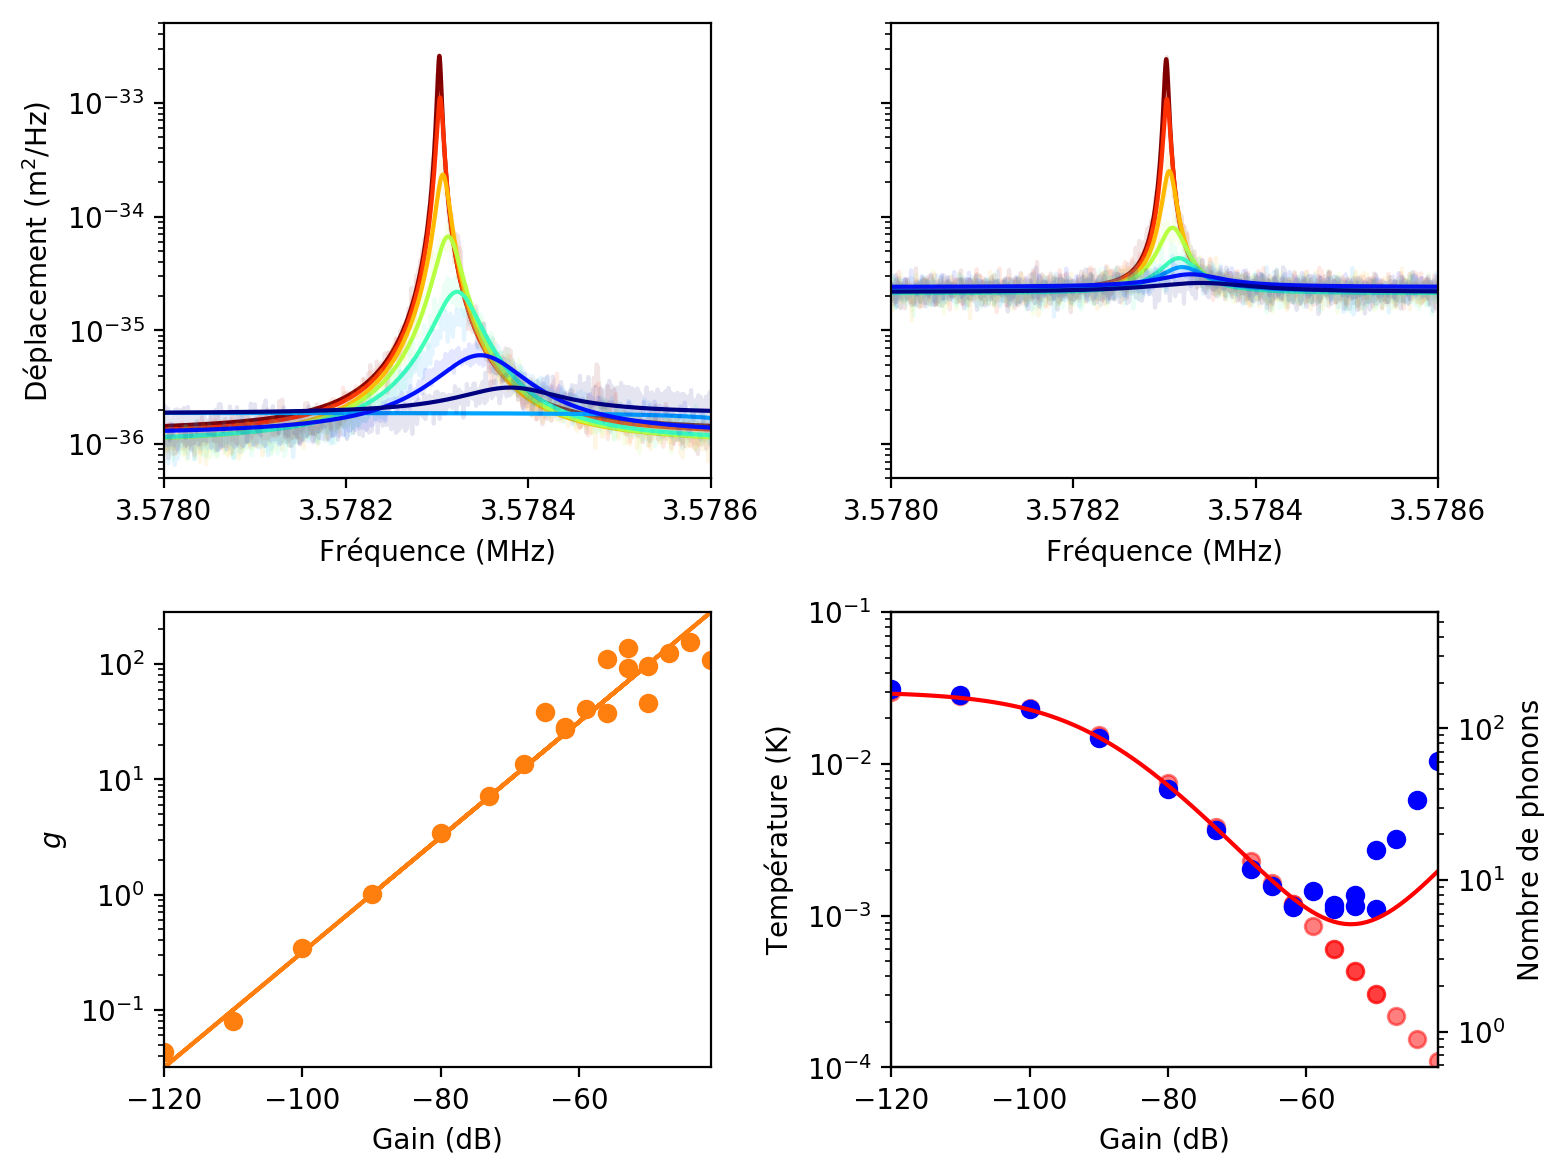
\includegraphics[scale=0.75]{figures/feedback_cooling_6phonons_defense_with_gain_all.png}
\caption{Refroidissement d'un micro-pilier proche de son état quantique fondamental.
En haut à gauche : spectres du bruit de position obtenus avec la détection homodyne donnant le signal d'erreur pour la boucle de rétroaction.
A droite, spectres obtenus avec la détection PDH indépendante de la boucle.
Les deux mesures sont réalisées simultanément.
Les données expérimentales sont tracées en transparence, l'ajustement par le modèle théorique correspond aux courbes pleines avec en rouge le gain le plus faible (correspondant à la température sans refroidissement par rétroaction) et en bleu la courbe obtenue pour le gain optimal correspondant à la température effective la plus faible.
En bas à gauche : gain extrait de l'ajustement des spectres homodyne en fonction du gain analogique.
A droite, températures effectives déduites des valeurs du gain en rouge (cas idéal) et des spectres PDH (en bleu).
La courbe rouge correspond au modèle qui tient compte des paramètres de l'expérience.
}
\label{fig:feedback_cooling_pillar}
\end{figure}

\section{Enseignement, diffusion et vulgarisation}

approche expérimentale

\subsection{Enseignements}

\subsection{Vulgarisation autour des ondes gravitationnelles}

Au cours de mes quatre années de thèse, j'ai eu l'occasion à plusieurs reprises de
\emph{Ce sujet, complètement d'actualité, pourrait faire l'objet d'une séquence pédagogique :
\begin{itemize}
\item sur le binaire d'Hulse et Taylor, rapprochement entre l'électrostatique et la gravitation, modèle de l'électron élastiquement lié pour modéliser le rayonnement gravitationnel et obtenir quelques ordres de grandeur ;
\item étude des barres résonantes de Weber, avec un modèle masse ressort (oscillateur harmonique faiblement amorti), pour en dégager les limitations (bande passante, sensibilité, etc.)
\item étude des interféromètres actuels (Michelson, Fabry Perot), des systèmes d'isolation (pendules, vide), boucle d'asservissement, traitement du signal.
\end{itemize}
}

\subsection{Aïkido}

%\bibliographystyle{custom-bib/thesis}
\bibliographystyle{abbrv}
\nocite{*}
\bibliography{biblio}

\end{document}